%%%%%%%%%%%%%%%%%%%%% chapter.tex %%%%%%%%%%%%%%%%%%%%%%%%%%%%%%%%%
%
% sample chapter
%
% Use this file as a template for your own input.
%
%%%%%%%%%%%%%%%%%%%%%%%% Springer-Verlag %%%%%%%%%%%%%%%%%%%%%%%%%%
%\motto{Use the template \emph{chapter.tex} to style the various elements of your chapter content.}
\chapter{Event Tree and Fault Tree Analysis}
\label{faulteventreechapter} % Always give a unique label
% use \chaptermark{}
% to alter or adjust the chapter heading in the running head
\chapterauthor{Bryan T. Adey and Nam Lethanh}
\section{Event tree analysis - Theory}
\subsection{Definition}
Event tree analysis (ETA) is a way to analyse and display different discrete
scenarios, their corresponding probability of occurrence and the resulting
consequences. ETA uses Boolean logic to analyse a chronological sequence of
events and estimate the probability of their occurrence. A key component of event
tree analysis is the event tree. An event tree is built from a starting event and
branches at each subsequent event based on the values of key parameters these key
parameters were intensity measures. When the event tree is complete, it is a
logical and visual representation of the set of scenarios that can occur, i.e.
multiple possible futures. An example is shown in Figure \ref{figeventfault:1}, the
initiating event is a 100-year precipitation, which may result in the occurrence
of a flood with water depths over 30 cm, under 30 cm, or not at all. In this
example, the flood can lead to different damage states related to an
infrastructure element, which can result in interruptions to traffic flow on the
road network. The consequences of the scenarios can then be quantified. Also the
heavy rain itself can cause an interruption.
\begin{figure}[h]
% \begin{center}
\includegraphics[width=300pt]{faulteventtree-1.eps}
\caption{Simplified event tree for a flood risk analysis}\label{figeventfault:1}
% \end{center}
\end{figure}
ETA is often referred to as having forward logic as it starts from an initiating
event and ends at a consequence. It is often used to analyze the risks associated
with systems, and the consequences of functioning or failed systems given that an
event(s) has (have) occurred. Simply the construction of an event tree can often
be useful in decision situations as it brings to light many scenarios that
decision makers otherwise would not have considered.

When conducting an ETA it is necessary to first determine the starting events
that are to be considered and then to think through each of the next possible
events to be considered. Each chain of events from initiating events to the end
event (or consequence) is referred to as a path, and may be thought of as a
scenario.

At each node in the event tree, the tree branches. There are often only two
branches that emanate from a node but it is possible that no split occurs or that
many splits occur. It is, however, of utmost importance to ensure that the split
represents mutually exclusive possibilities, i.e. if one possibility happens the
other cannot happen. The end events are often referred to as consequences.

The construction of an event tree requires knowledge about the system.
\subsection{Steps}


The basic steps to conduct an event tree analysis are:
\begin{enumerate}
\item Define static system: Determine what you would like to model and what is not to
be considered in the model
\item Define dynamic system: Determine what you would like to model over time. For
example, what hazards are of particular concern, e.g. flooding, what physical
things may happen, e.g. bridge collapse, what consequences might occur, e.g.
horrendous increases in travel times due to traffic jams
\item Identify specific initiating events: For example, heavy rain fall.
\item Identify specific intermediate events: For example, overtopping of a bridge
\item Construct the event tree
\item Calculate the probabilities of occurrence of each event: One possibility is
using fault tree analysis.
\item Calculate the probability of occurrence of each scenario or path:
\item Calculate the overall risk:
\item Evaluate the acceptability of the risk associated with each scenario and
overall:
\end{enumerate}
%
Due to the almost infinite number of ways to represent reality and the almost
infinite number of events that can occur, an appropriate system representation
needs to be developed. A good starting point is often the system representation
used to determine that there was a problem. It needs, however, to be verified
that this representation is adequate for the evaluation of the candidate
strategies. The necessary detail to be used depends on the specific question, the
strategies to be evaluated and the level of detail desired.
\subsection{Example in literature}
Please read the research work of \cite{Beim1997}, who constructed a event
tree analysis for a lock gate system, as part of the script.
\section{Event tree analysis - Example}
\subsection{Question A}
You are the road manager responsible for a particularly risky section of road.
It consists of a bridge that crosses a river and is just below a steep
embankment, upon which it is known that avalanches sometimes occur. This is
illustrated in Figure \ref{figfaultevent2x}.
%
\begin{figure}
 \begin{minipage}[h]{0.5\linewidth}
        \centering
        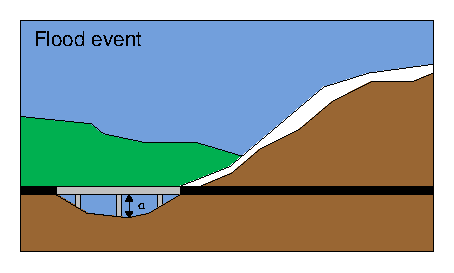
\includegraphics[scale=0.95]{faulteventtree-31.eps}
				\subcaption{Flood event}\label{faulteventtree-31}
     \end{minipage}
\vspace{3.00mm}
    \begin{minipage}[h]{0.5\linewidth}
       \centering
       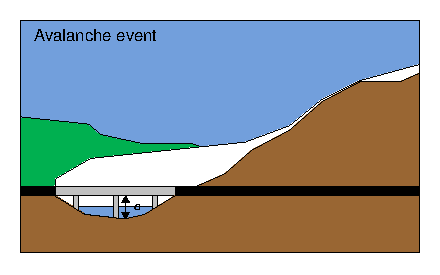
\includegraphics[scale=0.95]{faulteventtree-32.eps}
			\subcaption{Avalanche event}\label{faulteventtree-32}
     \end{minipage}
\caption{Illustration of risks}
\label{figfaultevent2x}
\end{figure}
%
You suspect that there are substantial infrastructure related risks due to both
flooding and avalanches but would like to quantify the risks. Develop an event
tree to allow you to do this.
\subsection{Answer A}
One of the first things to do when developing an event tree to allow you to
estimate the infrastructure related risks due to flooding and avalanches is to
determine the what will cause the branching in the event tree\footnote{The answer
is an adapted version of that used in \cite{Adey2009}}. The event tree is a part of the system
representation\footnote{The system representation is a model of the relevant part
of reality used for the evaluation and consists of all possible realizations of
stochastic processes within the investigated time period.}. The event tree in
this case should have sufficiently good representations of the structures,
hazards, and consequences, as well as the interaction between them so that it can
be reasonably certain that there is an appropriate understanding of the system
and that the risks. The event tree should consist of all possible things that can
happen in a specified period of time, i.e. scenarios. In the event tree a
scenario is represented by a path in the event tree. In the event tree proposed
here the paths are divided into five components, 1) event occurrence, 2) effect
of event, 3) physical changes in infrastructure, 4) direct consequences, and 5)
indirect consequences. An example for a bridge exposed to flooding and avalanches
is shown in Figure \ref{figeventfault:3}, assuming that flood and avalanche events are
mutually exclusive.
\begin{figure}[h]
\begin{center}
\includegraphics[width=300pt]{faulteventtree-13.eps}
\caption{Event tree with mutually exclusive flood and avalanche
events.}\label{figeventfault:3}
\end{center}
\end{figure}
In this event tree the hazard consists of the event and the effects on the
bridge object that are considered to have consequences. The effects on the bridge
are represented by two levels of the key parameters, water depth \textit{$>$= a
}and water depth \textit{$<$ a}, where \textit{a }is the bridge clearance, and
snow depth \textit{$>$= b }and snow depth \textit{$<$ b}, where \textit{b }is the
depth of snow on the bridge.

The consequence portion of the event tree is composed of the non-monetarisable
and monetarisable direct and indirect consequences. For each level of the key
parameter, assumptions are made with respect to the non-monetarisable direct
consequences that can occur, e.g. the physical behavior of the structure when the
specified level of the key parameter(s) occurs. The effect on the structure
should be described with the fewest possible parameters. Assumptions are made
with respect to the monetarisable direct consequences that can occur for each
non-monetarisable direct consequence, e.g. the fatalities related to the collapse
of the bridge. Assumptions are made with respect to the monetarisable indirect
consequences that can occur for each monetarisable direct consequence, e.g. the
additional user traffic time due to a deviation. The monetarisable consequences
can be attributed to those that will carry the consequences if failure occurs and
can be grouped by consequences type.
In the event tree (Figure \ref{figeventfault:3}), each effect has two possible
non-monetarisable direct consequences (\textit{nmDC{\tiny 1}, nmDC{\tiny 2}}).
For example, when the water depth during a flood is \textit{$>$= a}, than the two
possible failure modes are the wash out of the abutments (\textit{nmDC{\tiny 1}})
and the wash out of the columns (\textit{nmDC{\tiny 2}}). The monetarisable
direct consequences deterministically follow the non monetarisable direct
consequences (\textit{nmDC{\tiny 1}}). The monetarisable indirect consequences
are branched into the monetarisable indirect consequences that would occur if the
abutments were washed out during winter with low traffic volumes
(\textit{mIC{\tiny 1}}) and those that would occur if the abutments were washed
out during summer with high traffic volumes (\textit{mIC{\tiny 2}})
\subsection{Question B}
Construct an event tree for a road segment and a bridge that may be affected by
a flood or an avalanche, but not at the same time.
\subsection{Answer B}
The branches in the event tree are comprised of a chain of possible events and
monetarisable direct and indirect consequences (Fig. \ref{figeventfault:3} and Fig. \ref{figeventfault:4}). A slightly more
detailed example of some of the avalanche scenarios is given in Table
\ref{tbleventfault:1}, where the effect on the physical object is listed simply as level.
It is easy to imagine how detailed this can become.
\begin{figure}[h]
\begin{center}
\includegraphics[width=300pt]{faulteventtree-14.eps}
\caption{Event tree with mutually exclusive flood event.}\label{figeventfault:3}
\end{center}
\end{figure}

\begin{figure}[h]
\begin{center}
\includegraphics[width=300pt]{faulteventtree-15.eps}
\caption{Event tree with mutually exclusive avalanche event.}
\label{figeventfault:4}
\end{center}
\end{figure}

\begin{table}
	\centering
	\caption{Examples of scenarios} \label{tbleventfault:1}
\begin{tabular}{|c|c|c|c|}
\hline
Nr. & Effect & Non-monetarisable direct consequences & Monetarisable direct consequences \\ 
\hline
1 &  & Mild deformation of road surface & Level 1 \\ 
\cline{1-1}\cline{4-4}
2 &  &  & Level 2 \\ 
\cline{1-1}\cline{3-4}
3 &  & Severe deformation of road surface & Level 1 \\ 
\cline{1-1}\cline{4-4}
4 & On column level 1 &  & Level 2 \\ 
\cline{1-1}\cline{3-4}
5 &  & Collapse of object & Level 2 \\ 
\cline{1-1}\cline{4-4}
6 &  &  & Level 3 \\ 
\hline
- & - & - & - \\ 
- & - & - & - \\ 
- & - & - & - \\ 
\hline
31 &  & Mild displacement of deck & Level 1 \\ 
\cline{1-1}\cline{4-4}
32 &  &  & Level 2 \\ 
\cline{1-1}\cline{3-4}
33 &  & Severe displacement of deck & Level 1 \\ 
\cline{1-1}\cline{4-4}
34 & Horizontal loading of deck level 3 &  & Level 2 \\ 
\cline{1-1}\cline{3-4}
35 &  & Removal of superstructure & Level 2 \\ 
\cline{1-1}\cline{4-4}
36 &  &  & Level 3 \\ 
\hline
\end{tabular}
\end{table}
\subsection{Question C}
As a road manager you are considering the construction of avalanche protection
to reduce the infrastructure related risk.

You know that with respect to the probabilities of occurrence of events that
\begin{itemize}
\item if you do nothing,the probability of occurrence of an avalanche decreases from
0.5 in 2009 to 0.3 in 2029 due to ever decreasing snow fall.
\item If you construct avalanche protection, the probability of occurence of an
avalanche will be 0 for the next 10 years but will increase after that
\end{itemize}
You know that the conditional probabilities of the effects on the loading of the
column, the horizontal loading of the superstructure and the vertical loading of
the superstructure are constant and as shown in Table \ref{tbleventfault:2}. You know that
conditional probability of physical changes due to horizontal loading of the
columns and deck increases by 0.001 per year to take into account normal
deterioration (Table \ref{tbleventfault:3} and Table \ref{tbleventfault:4}) and due to vertical
loading of deck is 1 and constant (Table \ref{tbleventfault:5}). You also know that the due
to changes in traffic that the conditional probabilities of consequences are as
shown in Table \ref{tbleventfault:6}. You have also estimate the consequences of each
consequence level to be those as shown in Table \ref{tbleventfault:7}.

Is it worth it if only a 20 year horizon is analysed?  (Use a discount factor of
2\%. Assume that the probability of multiple failures of the same infrastructure
object are negligible. Show the yearly costs and benefits as well as the totals.
For simplicity, assume that there is only one level of monetarisable consequences
per level of physical damage.)

\begin{table}
	\centering
	\caption{Conditional probabilities of the effects} \label{tbleventfault:2}
\begin{tabular}{|l|l|l|l|l|l|l|l|l|l|}
\hline
\multicolumn{1}{|c|}{Year} & \multicolumn{3}{c|}{Loading of the column} & \multicolumn{3}{m{2.5cm}|}{\centering Horizontal loading of the superstructure} & \multicolumn{3}{m{2.5cm}|}{\centering Vertical loading of the superstructure} \\ 
\cline{2-10}
\multicolumn{1}{|c|}{} & \multicolumn{1}{c|}{Level 1} & \multicolumn{1}{c|}{Level 2} & \multicolumn{1}{c|}{Level 3} & \multicolumn{1}{c|}{Level 1} & \multicolumn{1}{c|}{Level 2} & \multicolumn{1}{c|}{Level 3} & \multicolumn{1}{c|}{Level 1} & \multicolumn{1}{c|}{Level 2} & \multicolumn{1}{c|}{Level 3} \\ 
\hline
\multicolumn{1}{|c|}{2009} & \multicolumn{1}{c|}{0.3} & \multicolumn{1}{c|}{0.4} & \multicolumn{1}{c|}{0.3} & \multicolumn{1}{c|}{0.3} & \multicolumn{1}{c|}{0.4} & \multicolumn{1}{c|}{0.3} & \multicolumn{1}{c|}{0.3} & \multicolumn{1}{c|}{0.4} & \multicolumn{1}{c|}{0.3} \\ 
\hline
\multicolumn{1}{|c|}{2010} & \multicolumn{1}{c|}{0.3} & \multicolumn{1}{c|}{0.4} & \multicolumn{1}{c|}{0.3} & \multicolumn{1}{c|}{0.3} & \multicolumn{1}{c|}{0.4} & \multicolumn{1}{c|}{0.3} & \multicolumn{1}{c|}{0.3} & \multicolumn{1}{c|}{0.4} & \multicolumn{1}{c|}{0.3} \\ 
\hline
\multicolumn{1}{|c|}{2011} & \multicolumn{1}{c|}{0.3} & \multicolumn{1}{c|}{0.4} & \multicolumn{1}{c|}{0.3} & \multicolumn{1}{c|}{0.3} & \multicolumn{1}{c|}{0.4} & \multicolumn{1}{c|}{0.3} & \multicolumn{1}{c|}{0.3} & \multicolumn{1}{c|}{0.4} & \multicolumn{1}{c|}{0.3} \\ 
\hline
\multicolumn{1}{|c|}{2012} & \multicolumn{1}{c|}{0.3} & \multicolumn{1}{c|}{0.4} & \multicolumn{1}{c|}{0.3} & \multicolumn{1}{c|}{0.3} & \multicolumn{1}{c|}{0.4} & \multicolumn{1}{c|}{0.3} & \multicolumn{1}{c|}{0.3} & \multicolumn{1}{c|}{0.4} & \multicolumn{1}{c|}{0.3} \\ 
\hline
\multicolumn{1}{|c|}{2013} & \multicolumn{1}{c|}{0.3} & \multicolumn{1}{c|}{0.4} & \multicolumn{1}{c|}{0.3} & \multicolumn{1}{c|}{0.3} & \multicolumn{1}{c|}{0.4} & \multicolumn{1}{c|}{0.3} & \multicolumn{1}{c|}{0.3} & \multicolumn{1}{c|}{0.4} & \multicolumn{1}{c|}{0.3} \\ 
\hline
\multicolumn{1}{|c}{-} & \multicolumn{1}{c}{-} & \multicolumn{1}{c}{-} & \multicolumn{1}{c}{-} & \multicolumn{1}{c}{-} & \multicolumn{1}{c}{-} & \multicolumn{1}{c}{-} & \multicolumn{1}{c}{-} & \multicolumn{1}{c}{-} & \multicolumn{1}{c|}{-} \\ 
\multicolumn{1}{|c}{-} & \multicolumn{1}{c}{-} & \multicolumn{1}{c}{-} & \multicolumn{1}{c}{-} & \multicolumn{1}{c}{-} & \multicolumn{1}{c}{-} & \multicolumn{1}{c}{-} & \multicolumn{1}{c}{-} & \multicolumn{1}{c}{-} & \multicolumn{1}{c|}{-} \\ 
\hline
\multicolumn{1}{|c|}{2025} & \multicolumn{1}{c|}{0.3} & \multicolumn{1}{c|}{0.4} & \multicolumn{1}{c|}{0.3} & \multicolumn{1}{c|}{0.3} & \multicolumn{1}{c|}{0.4} & \multicolumn{1}{c|}{0.3} & \multicolumn{1}{c|}{0.3} & \multicolumn{1}{c|}{0.4} & \multicolumn{1}{c|}{0.3} \\ 
\hline
\multicolumn{1}{|c|}{2026} & \multicolumn{1}{c|}{0.3} & \multicolumn{1}{c|}{0.4} & \multicolumn{1}{c|}{0.3} & \multicolumn{1}{c|}{0.3} & \multicolumn{1}{c|}{0.4} & \multicolumn{1}{c|}{0.3} & \multicolumn{1}{c|}{0.3} & \multicolumn{1}{c|}{0.4} & \multicolumn{1}{c|}{0.3} \\ 
\hline
\multicolumn{1}{|c|}{2027} & \multicolumn{1}{c|}{0.3} & \multicolumn{1}{c|}{0.4} & \multicolumn{1}{c|}{0.3} & \multicolumn{1}{c|}{0.3} & \multicolumn{1}{c|}{0.4} & \multicolumn{1}{c|}{0.3} & \multicolumn{1}{c|}{0.3} & \multicolumn{1}{c|}{0.4} & \multicolumn{1}{c|}{0.3} \\ 
\hline
\multicolumn{1}{|c|}{2028} & \multicolumn{1}{c|}{0.3} & \multicolumn{1}{c|}{0.4} & \multicolumn{1}{c|}{0.3} & \multicolumn{1}{c|}{0.3} & \multicolumn{1}{c|}{0.4} & \multicolumn{1}{c|}{0.3} & \multicolumn{1}{c|}{0.3} & \multicolumn{1}{c|}{0.4} & \multicolumn{1}{c|}{0.3} \\ 
\hline
\multicolumn{1}{|c|}{2029} & \multicolumn{1}{c|}{0.3} & \multicolumn{1}{c|}{0.4} & \multicolumn{1}{c|}{0.3} & \multicolumn{1}{c|}{0.3} & \multicolumn{1}{c|}{0.4} & \multicolumn{1}{c|}{0.3} & \multicolumn{1}{c|}{0.3} & \multicolumn{1}{c|}{0.4} & \multicolumn{1}{c|}{0.3} \\ 
\hline
\end{tabular}
\end{table}

\begin{table}
	\centering
	\caption{Conditional probabilities of the occurrence of the physical changes due to loading of the column} \label{tbleventfault:3}
\begin{tabular}{|c|c|c|c|}
\hline
Year & \multicolumn{3}{c|}{Effect} \\ 
\cline{2-4}
 & \multicolumn{3}{c|}{Loading of column} \\ 
\cline{2-4}
 & Mild deformation of road surface & Severe deformation of road surface & Collapse of object \\ 
\hline
2009 & 0.2 & 0.2 & 0.2 \\ 
\hline
2010 & 0.201 & 0.201 & 0.201 \\ 
\hline
2011 & 0.202 & 0.202 & 0.202 \\ 
\hline
2012 & 0.203 & 0.203 & 0.203 \\ 
\hline
- & - & - & - \\ 
- & - & - & - \\ 
\hline
2027 & 0.218 & 0.218 & 0.218 \\ 
\hline
2028 & 0.219 & 0.219 & 0.219 \\ 
\hline
2029 & 0.220 & 0.220 & 0.220 \\ 
\hline
\end{tabular}
\end{table}

\begin{table}
	\centering
	\caption{Conditional probabilities of the occurrence of the physical changes due to horizontal loading of the deck} \label{tbleventfault:4}
\begin{tabular}{|c|c|c|c|}
\hline
Year & \multicolumn{3}{c|}{Effect} \\ 
\cline{2-4}
 & \multicolumn{3}{c|}{Horizontal loading of deck} \\ 
\cline{2-4}
 & Mild deformation of road surface & Severe deformation of road surface & Collapse of object \\ 
\hline
2009 & 0.2 & 0.2 & 0.2 \\ 
\hline
2010 & 0.201 & 0.201 & 0.201 \\ 
\hline
2011 & 0.202 & 0.202 & 0.202 \\ 
\hline
2012 & 0.203 & 0.203 & 0.203 \\ 
\hline
- & - & - & - \\ 
- & - & - & - \\ 
\hline
2027 & 0.218 & 0.218 & 0.218 \\ 
\hline
2028 & 0.219 & 0.219 & 0.219 \\ 
\hline
2029 & 0.220 & 0.220 & 0.220 \\ 
\hline
\end{tabular}
\end{table}

\begin{table}
	\centering
	\caption{Conditional probabilities of the occurrence of the physical changes due to vertical loading of the deck} \label{tbleventfault:5}
\begin{tabular}{|c|c|c|c|}
\hline
Year & \multicolumn{3}{c|}{Effect} \\ 
\cline{2-4}
 & \multicolumn{3}{c|}{Vertical loading of deck} \\ 
\cline{2-4}
 & Slightly yielded reinforcement & Plasticized reinforcement & Collapse of object \\ 
\hline
2009 & 1 & 1 & 1 \\ 
\hline
2010 & 1 & 1 & 1 \\ 
\hline
2011 & 1 & 1 & 1 \\ 
\hline
2012 & 1 & 1 & 1 \\ 
\hline
- & - & - & - \\ 
- & - & - & - \\ 
\hline
2027 & 1 & 1 & 1 \\ 
\hline
2028 & 1 & 1 & 1 \\ 
\hline
2029 & 1 & 1 & 1 \\ 
\hline
\end{tabular}
\end{table}

\begin{table}
	\centering
	\caption{Conditional probabilities of monetarisable (direct and indirect) consequences} \label{tbleventfault:6}
\begin{tabular}{|l|l|l|l|l|l|l|l|l|}
\hline
\multicolumn{1}{|c|}{Year} & \multicolumn{4}{m{4.5cm}|}{\centering Loading of column (L1, L2, L3) Horizonal loading of deck} & \multicolumn{2}{m{2cm}|}{\centering Vertical loading of deck (L1, L2)} & \multicolumn{2}{m{2cm}|}{\centering Vertical load of deck (L3)} \\ 
\cline{2-9}
\multicolumn{1}{|c|}{} & \multicolumn{8}{c|}{Failure mode} \\ 
\cline{2-9}
\multicolumn{1}{|c|}{} & \multicolumn{2}{m{2cm}|}{\centering Deformation of road surface} & \multicolumn{2}{m{2cm}|}{\centering Collapse of object} & \multicolumn{2}{m{2cm}|}{\centering Slightly yielded / plastized rebar} & \multicolumn{2}{m{2cm}|}{\centering Collapse of object} \\ 
\cline{2-9}
\multicolumn{1}{|c|}{} & \multicolumn{8}{c|}{Monetarisable direct and indirect consequences} \\ 
\cline{2-9}
\multicolumn{1}{|c|}{} & \multicolumn{1}{c|}{Level 1} & \multicolumn{1}{c|}{Level 2} & \multicolumn{1}{c|}{Level 1} & \multicolumn{1}{c|}{Level 2} & \multicolumn{1}{c|}{Level 1} & \multicolumn{1}{c|}{Level 2} & \multicolumn{1}{c|}{Level 2} & \multicolumn{1}{c|}{Level 3} \\ 
\hline
\multicolumn{1}{|c|}{2009} & \multicolumn{1}{c|}{0.5} & \multicolumn{1}{c|}{0.5} & \multicolumn{1}{c|}{0.5} & \multicolumn{1}{c|}{0.5} & \multicolumn{1}{c|}{0.5} & \multicolumn{1}{c|}{0.5} & \multicolumn{1}{c|}{0.5} & \multicolumn{1}{c|}{0.5} \\ 
\hline
\multicolumn{1}{|c|}{2010} & \multicolumn{1}{c|}{0.499} & \multicolumn{1}{c|}{0.501} & \multicolumn{1}{c|}{0.499} & \multicolumn{1}{c|}{0.501} & \multicolumn{1}{c|}{0.499} & \multicolumn{1}{c|}{0.501} & \multicolumn{1}{c|}{0.499} & \multicolumn{1}{c|}{0.501} \\ 
\hline
\multicolumn{1}{|c|}{2011} & \multicolumn{1}{c|}{0.498} & \multicolumn{1}{c|}{0.502} & \multicolumn{1}{c|}{0.498} & \multicolumn{1}{c|}{0.502} & \multicolumn{1}{c|}{0.498} & \multicolumn{1}{c|}{0.502} & \multicolumn{1}{c|}{0.498} & \multicolumn{1}{c|}{0.502} \\ 
\hline
\multicolumn{1}{|c}{-} & \multicolumn{1}{c}{-} & \multicolumn{1}{c}{-} & \multicolumn{1}{c}{-} & \multicolumn{1}{c}{-} & \multicolumn{1}{c}{-} & \multicolumn{1}{c}{-} & \multicolumn{1}{c}{-} & \multicolumn{1}{c|}{-} \\ 
\multicolumn{1}{|c}{-} & \multicolumn{1}{c}{-} & \multicolumn{1}{c}{-} & \multicolumn{1}{c}{-} & \multicolumn{1}{c}{-} & \multicolumn{1}{c}{-} & \multicolumn{1}{c}{-} & \multicolumn{1}{c}{-} & \multicolumn{1}{c|}{-} \\ 
\hline
\multicolumn{1}{|c|}{2027} & \multicolumn{1}{c|}{0.482} & \multicolumn{1}{c|}{0.518} & \multicolumn{1}{c|}{0.482} & \multicolumn{1}{c|}{0.518} & \multicolumn{1}{c|}{0.482} & \multicolumn{1}{c|}{0.518} & \multicolumn{1}{c|}{0.482} & \multicolumn{1}{c|}{0.518} \\ 
\hline
\multicolumn{1}{|c|}{2028} & \multicolumn{1}{c|}{0.481} & \multicolumn{1}{c|}{0.519} & \multicolumn{1}{c|}{0.481} & \multicolumn{1}{c|}{0.519} & \multicolumn{1}{c|}{0.481} & \multicolumn{1}{c|}{0.519} & \multicolumn{1}{c|}{0.481} & \multicolumn{1}{c|}{0.519} \\ 
\hline
\multicolumn{1}{|c|}{2029} & \multicolumn{1}{c|}{0.480} & \multicolumn{1}{c|}{0.520} & \multicolumn{1}{c|}{0.480} & \multicolumn{1}{c|}{0.520} & \multicolumn{1}{c|}{0.480} & \multicolumn{1}{c|}{0.520} & \multicolumn{1}{c|}{0.480} & \multicolumn{1}{c|}{0.520} \\ 
\hline
\end{tabular}
\end{table}

\begin{table}
	\centering
	\caption{Consequences} \label{tbleventfault:7}
\begin{tabular}{|p{2cm}|p{2.5cm}|c|c|c|c|c|c|c|}
\hline
Effect & Physical change & Level 1 & \multicolumn{2}{c|}{Owner} & \multicolumn{2}{c|}{User} & \multicolumn{2}{c|}{Public} \\ 
\cline{4-9}
 &  &  & Inter-vention & Travel time & Nr. injuries & Nr. fatal-ities & Nr. injuries & Nr. fatal-ities \\ 
\cline{4-9}
 &  &  & 106 CHF & 106 CHF & 106 CHF & 106 CHF & 106 CHF & 106 CHF \\ 
\hline
On column level 1, 2 and 3 & None & None & 0 & 0 & 0 & 0 & 0 & 0 \\ 
\cline{2-9}
 & Light deformation  of road surface & 1 & 0 & 0 & 0 & 0 & 0 & 0 \\ 
\cline{3-9}
 &  & 2 & 0.5 & 0.5 & 0.5 & 0.5 & 0.5 & 0.5 \\ 
\cline{2-9}
 & Mild deformation of road surface & 1 & 1.5 & 1.5 & 1.5 & 1.5 & 1.5 & 1.5 \\ 
\cline{3-9}
 &  & 2 & 2.5 & 2.5 & 2.5 & 2.5 & 2.5 & 2.5 \\ 
\cline{2-9}
 & Collapse of object & 2 & 5 & 5 & 5 & 5 & 5 & 5 \\ 
\cline{3-9}
 &  & 3 & 10 & 10 & 10 & 10 & 10 & 10 \\ 
\hline
 &  & - & - & - & - & - & - & - \\ 
\hline
Vertical loading of deck Stufe 3 & Collapse of object & 2 & 1 & 1 & 1 & 1 & 1 & 1 \\ 
\cline{3-9}
 &  & 3 & 2.5 & 2.5 & 2.5 & 2.5 & 2.5 & 2.5 \\ 
\hline
\end{tabular}
\end{table}
\subsection{Answer C}
The breakdown of the relative costs and benefits is given in Table \ref{tbleventfault:8}.
The yearly costs and benefits are given in Figure \ref{figeventfault:4}-Figure \ref{figeventfault:5}.
The avalanche protection should be built.
\begin{table}
	\centering
	\caption{ Costs, benefits and effectiveness} \label{tbleventfault:8}
\begin{tabular}{|c|p{1.2cm}|p{1.5cm}|c|p{1.5cm}|p{1.5cm}|c|c|}
\hline
Intervention & \multicolumn{3}{c|}{Relative costs ($10^6$ mu)} & \multicolumn{3}{c|}{Relative benefits (106 mu)} & Effectiveness (B-C) \\ 
\cline{2-8}
 & \centering Planned interventions & \centering Restoration following failure & Total & \centering Reduction of material damage risks & \centering Reduction of failure risks & Total &  \\ 
\hline
Do nothing & \centering 0 & \centering 0 & \centering 0 & \centering 0 & \centering 0 & \centering 0 & 0 \\ 
\hline
Avalanche protection & \centering 4.00 & \centering -1.00 & \centering 3.00 & \centering 2.00 & \centering 3.00 & \centering 5.00 & 2.00 \\ 
\hline
\end{tabular}
\end{table}

\begin{figure}[h]
\begin{center}
\includegraphics[width=300pt]{faulteventtree-16.eps}
\caption{Discounted costs of intervention per year for the do nothing
intervention}\label{figeventfault:4}
\end{center}
\end{figure}

\begin{figure}[h]
\begin{center}
\includegraphics[width=300pt]{faulteventtree-17.eps}
\caption{Discounted risk per year for the do nothing intervention}
\end{center}
\end{figure}

\begin{figure}[h]
\begin{center}
\includegraphics[width=300pt]{faulteventtree-18.eps}
\caption{Discounted costs of intervention per year for the avalanche protection
intervention}
\end{center}
\end{figure}

\begin{figure}[h]
\begin{center}
\includegraphics[width=300pt]{faulteventtree-19.eps}
\caption{Discounted risk per year for the avalanche protection intervention}
\end{center}
\end{figure}

\begin{figure}[h]
\begin{center}
\includegraphics[width=300pt]{faulteventtree-20.eps}
\caption{Discounted benefit (in terms of risk reduction) per year for the
avalanche protection intervention}\label{figeventfault:5}
\end{center}
\end{figure}
\section{Fault tree analysis -- Theory}
\subsection{Definition}
Fault tree analysis is often used when it is desired to focus on the particular
ways a system can fail. It is particularly well suited to determine the
probability of a specific event happening when this event can happen due to
different precursor events. Fault trees are often used in the evaluation of large
safety-critical systems \citep{Andrews2012}.

Fault tree analysis is often referred to as having backward logic as specific
consequences are first determined and then the causes of these consequences are
worked out, i.e. working backwards in time. Fault tree analysis is also sometimes
seen as being top down, i.e. how can the top event be determined from a
combination of lower level events.

In the development of a fault tree one normally starts by defining a top event
and then developing logical expressions of sub-events that may lead to the
occurrence of the top event. The last events in the tree are base events, or
initiating events. Once a fault tree is constructed and the probability of
occurrence of the base events are estimated the probability of occurrence of the
top event can be estimated. When constructing fault trees it is necessary to
ensure that that the events are binary events e.g. failure or no failure, that
they are statistically independent, and that the relationships between events and
causes can be represented by means of logical gates.

Fault trees can also be used to assess the infrastructure related risk due to
natural hazards. Their focus, however, is more on a specific type of consequence,
which may happen due to hazard of different types, e.g. a bridge may collapse due
to a flood or an earthquake.

A separate fault tree is required for every separate top event, or in other
words every failure mode.
\subsection{Symbols}
A fault tree makes use of events and logic gates. These are shown in Table
\ref{tbleventfault:9} and Table \ref{tbleventfault:10}.
\begin{table}
\centering
\caption{Fault tree events} \label{tbleventfault:9}
\begin{tabular}{|>{\centering\arraybackslash}m{2cm}|>{\raggedright\arraybackslash}m{3.5cm}|c|}
\hline
Event label & Event description & Event symbol \\ 
\hline
Basic event & failure or error in a subitem & \includegraphics[scale=0.5]{faulteventtree-2.eps} \\ 
\hline
House event & The event is known to be true or false & \includegraphics[scale=0.5]{faulteventtree-3.eps} \\ 
\hline
Undeveloped event & An event about which insufficient information is available, or which is of no consequence & 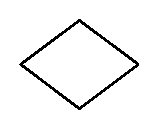
\includegraphics[scale=0.5]{faulteventtree-4.eps} \\ 
\hline
Conditional event & conditions that restrict or affect logic gates & 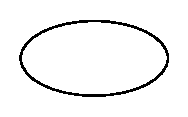
\includegraphics[scale=0.5]{faulteventtree-5.eps} \\ 
\hline
Intermediate event & can be used immediately above a primary event to provide more room to type the event description & 
\includegraphics[scale=0.5]{faulteventtree-6.eps} \\ 
\hline
\end{tabular}
\end{table}

\begin{table}
\centering
\caption{Fault tree logic gates} \label{tbleventfault:10}
\begin{tabular}{|>{\centering\arraybackslash}m{2cm}|>{\raggedright\arraybackslash}m{3.5cm}|>{\centering\arraybackslash}m{2cm}|}
\hline
Gate label & Gate description & Gate symbol \\ 
\hline
OR & the output occurs if any input occurs & 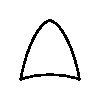
\includegraphics[scale=0.5]{faulteventtree-7.eps} \\ 
\hline
AND & the output occurs only if all inputs occur (inputs are independent) & 
\includegraphics[scale=0.5]{faulteventtree-8.eps} \\ 
\hline
Exclusive OR & the output occurs if exactly one input occurs & 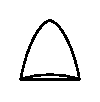
\includegraphics[scale=0.5]{faulteventtree-9.eps} \\ 
\hline
Priority AND & the output occurs if the inputs occur in a specific sequence specified by a conditioning event & \includegraphics[scale=0.5]{faulteventtree-10.eps} \\ 
\hline
Inhibit & the output occurs if the input occurs under an enabling condition specified by a conditioning event & \includegraphics[scale=0.5]{faulteventtree-11.eps} \\ 
\hline
Voting & output event occurs if at least m of the input occur & \includegraphics[scale=0.5]{faulteventtree-12.eps} \\ 
\hline
\end{tabular}
\end{table}
%
\subsection{Steps}
FTA analysis involves five steps:
\begin{enumerate}
\item Define the undesired event, i.e. the top event.
\item Obtain an understanding of the system, i.e. determine all possible ways that
this undesired event may happen. This requires experts who understand the
functioning of the system well. If something is overlooked it will not be
included in the fault tree and this may result in less than optimal decision
being made to reduce the probability of occurrence of the undesired event.
\item Construct the fault tree:
\item Evaluate the fault tree: this requires the determination or estimation of the
probability of occurrence of all base events and then the estimation of the
probability of occurrence of the top event. As the determination of the
probability of occurrence of all base events may take considerable time and
effort it is worthwhile to keep in mind the exactness required so that a decision
maker can come to the optimal decision. This estimation of the probability of the
occurrence of the top event. This is explained in week 9 ``Performance
indicators: Reliability''.
\end{enumerate}
\subsection{Examples in literature}
FTA has been widely used in management of many infrastructure systems. Some of
examples are with gas system \cite{Andrews2012,Tian2012}; bridges \cite{Davis-McDaniel2013,Johnson1999,Sianipar1997,LeBeau2007}; tunneling \cite{You2012}, and urban transport \cite{Ma2014}. Students are requested to read these cited works as part of the handout.
\section{Fault tree analysis -- Example B}
\subsection{Question B1}
As the manager of the bridge shown in Figure \ref{figeventfault:6} and Figure \ref{figeventfault:7},
you are interested in having an overview of all the ways it might fail so you can
determine the most effective way for you to reduce your risks. Construct a
failure tree covering the following hazards 1) corrosion of the steel
reinforcement, 2) spalling of concrete, 3) corrosion of the steel beams, 4)
fatigue of the steel beams, 5) fire, 6) train impact, 7) over loading due to
vehicles, 8) earthquakes, 9) scour. Assume the top event to be bridge collapse.

\begin{figure}[h]
\begin{center}
\includegraphics[width=352pt]{faulteventtree-22.eps}
\caption{Getwing bridge}\label{figeventfault:6}
\end{center}
\end{figure}


\begin{figure}[h]
\begin{center}
\includegraphics[scale=1.5]{faulteventtree-23.eps}
\caption{Design of Getwing bridge}\label{figeventfault:7}
\end{center}
\end{figure}

\subsection{Answer B1}


A possible fault tree for the case of bridge collapse can be constructed and
shown in following figures.

\begin{figure}[h]
\begin{center}
\includegraphics[scale=0.6]{faulteventtree-24.eps}
\caption{First level of the fault tree}\label{figeventfault:8}
\end{center}
\end{figure}

In Figure \ref{figeventfault:8}, the first level of the fault tree is shown. The bridge
can collapse due to the collapse of either the superstructure (beams, girders) or
the substructures (abutment and piers). The failure of both superstructure and
the substructures are developed in the next figures.

\begin{figure}[h]
\begin{center}
\includegraphics[scale=0.6]{faulteventtree-25.eps}
\caption{Second level of the fault tree (superstructure)}\label{figeventfault:9}
\end{center}
\end{figure}

Figure \ref{figeventfault:9} shows the cause of the failure of superstructure can be due to the
failure of the beams or girders (elements). Furthermore, the failure of each
element can be, either due to manifest deterioration processes or latent
deterioration processes.

\begin{figure}[h]
\begin{center}
\includegraphics[scale=0.6]{faulteventtree-26.eps}
\caption{Second level of the fault tree (sub-structures)}\label{figeventfault:10}
\end{center}
\end{figure}

Similar to Figure \ref{figeventfault:9}, Figure \ref{figeventfault:10} shows the fault tree for the
substructure, which includes the piers, abutments and bearing system. For the
sake of simplicity, only three branches under sub-structure are shown. The full
diagram would include many more branches. For example, instead of considering the
failure of abutments as one event, the failure of each abutment may be considered
as a separate event, i.e. failure of abutment 1 and failure of abutment 2, and
therefore an illustration of this would include two more branches. Similarly, the
development of the fault tree for piers could include the failure of each pier as
a separate branch. The level of detail to be considered depends on the detail
required in the analysis and the amount of effort to be invested.

Figure \ref{figeventfault:11} shows the last step in development of the tree for the beam
that is affected by manifest processes, e.g. corrosion, cracking, and fatigue
under the normal traffic condition and no error in the design phase. There are a
set of mathematical models to capture these manifest deterioration process (see
script of week 4). It is noted that in this last step of tree development. The
round circle or rectangular is used. This step often involves with the estimation
of probability for the event to occur. For example, under the ``failure due to
corrosion of steels'', there are two direct event that can be consider: 1) the
first event is the concentration of chloride reaching a critical level of 0.48
(see script of week 4); 2) and other event could be the age of the bridge.
%
\begin{figure}[ht]
\begin{center}
\includegraphics[scale=0.8]{faulteventtree-27.eps}
\caption{Third level of the fault tree (superstructure-beam- manifest
process)}\label{figeventfault:11}
\end{center}
\end{figure}
%
\begin{figure}[ht]
\begin{center}
\includegraphics[scale=1]{faulteventtree-28.eps}
\caption{Third level of the fault tree (superstructure- latent process)}
\end{center}
\end{figure}
%
\begin{figure}[ht]
\begin{center}
\includegraphics[scale=1]{faulteventtree-29.eps}
\caption{Sub-structure (abutment)}
\end{center}
\end{figure}

The complete fault tree for this example is given in OpenFTA extension file.
Students are adviced to install an open source fault tree analysis software
called ``OpenFTA'' from following link \href{http://www.openfta.com/}{http://www.openfta.com/}.
\subsection{Question B2}
Expand the fault tree to investigate the failure due to scour of the foundation
of column 6.
\subsection{Answer B2}
This figure shows the extension of the fault tree, which includes the scouring
process affecting the abutments and the piers of the bridges. The scouring
process can be due to four process: 1) local scouring; 2) contraction; 3)
widening; and 4) lateral migration. To understand these terminology, students are
advised to read the work of \cite{Johnson1999}, which is provided as the class handout.

\begin{figure}[ht]
\begin{center}
\includegraphics[scale=1]{faulteventtree-30.eps}
\caption{Fault tree for scouring of the pier}
\end{center}
\end{figure}
\section{Assignment}
\subsection{Problem A: Event tree analysis}
Water is one of the fundamental needs of millions of people living in a
megacity. Water of sufficient quality and quantity must be provided around the
clock. In order to fulfill this need, a city depends on its water distribution
infrastructure, which includes pipes made of different materials and laid at
different times. These pipes are affected by processes of different types and
deteriorate at different rates. The consequences related to pipe failure vary
significantly depending on the type of failure, e.g. a pipe break, or a leaking
pipe, as does the reaction time required to fix the pipe. For example, if a pipe
breaks, an inadequate LOS occurs immediately and a corrective intervention is to
be executed very quickly, and if it is noticed that there is progressive water
loss over time then a preventive intervention can be planned before there is an
inadequate LOS. Part of the water distribution network in mega-city Q is shown in
Figure \ref{fig24}. The pipe characteristics are given in Table \ref{tbl:213}.

\subsubsection{Question A1}
Construct an event tree for the pipe network if an earthquake occurs? The event
tree should include a sensible classification of events and consequences and it
should be realistic to determine the probability of occurrence of each scenario.
For the example, you should assume a probability of occurrence of each event in
your event tree, and then estimate the probability of occurrence of each
scenario. At whatever level you define your event tree be sure that it is
complete!
\subsubsection{Answer A1}
No specific answer is provided. Please submit your answer to obtain feedback. A
possible source event is the occurrence of an earthquake. Possible intermediary
events are the zones in which a pipe breaks occur if an earthquake occurs.
Possible network events are the loss of water and the loss of water pressure to
serviced areas.
\section{Problem B1 }
The manager of the pipeline network as shown in Figure \ref{fig24} expects to
understand how a large amount of water loss could occur. Water loss can be due to
many reasons, which includes the manifest and latent deterioration process.
\subsection{Question B1}
Construct a fault tree for the pipe network (Figure \ref{fig24}) if there is a
massive amount of water loss?
\subsection{Answer B1}
No specific answer is provided. Please submit your answer to obtain feedback.
Keep in mind though that water loss may happen in one or more zones, and that
these zones could be subdivided into specific pipes. Keep in mind that there are
many different ways for pipes to fail, e.g. holes in pipes can occur due to
differential soil movements, due to the penetration of roots into the pipes, the
corrosion of reinforcement, sabotage, mistakes on construction sites, etc.

\bibliographystyle{plainnat}
\bibliography{reference}
% 